\section{Ruling Out Generic Prompt Sensitivity}
\label{sec:prompt-control}
The reward intervention changes the reflection instruction together with the reward semantics. A generic prompt-sensitivity account therefore predicts that a sufficiently strong wording perturbation inside one reflection mode should produce comparable memory divergence. We test that reduction on eight released trajectories disjoint from F0 and balanced across original outcomes.

Before provider calls, we freeze semantic-preserving rewordings for both reflection modes. Under token-set Jaccard distance, the released success-versus-failure prompts differ by 0.114. The within-success rewording differs by 0.171 and the within-failure rewording by 0.152. The control thus perturbs surface wording more strongly while preserving the reflection objective.

Each fresh trajectory is written with the released success mode and the released failure mode. The same writer also processes one frozen semantic-preserving rewording of each mode at temperature zero. Let $B_i$ be the memory distance between the two released reward modes and let $W_i$ be the mean within-mode rewording distance. The frozen paired statistic is
\begin{equation}
\Delta_{\mathrm{prompt}}=\frac{1}{8}\sum_{i=1}^{8}(B_i-W_i).
\end{equation}

\begin{figure}[t]
\centering
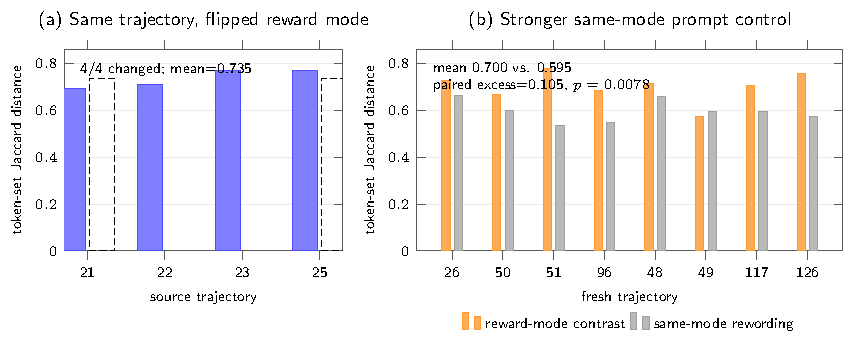
\includegraphics[width=\linewidth]{figures/fig2_write_and_prompt_control.pdf}
\caption{Write-channel evidence and its strongest simple control. (a) Among the four F0 pairs complete in both writer conditions, flipping only the reward-conditioned writer mode changes every memory. (b) On eight fresh control trajectories, reward-mode memory divergence exceeds stronger semantic-preserving same-mode prompt rewording. The control mean is 0.595 versus 0.700 between reward modes; paired excess is 0.105 with exact $p=0.0078$.}
\label{fig:write-control}
\end{figure}

All 32 control outputs complete. Mean reward-mode distance is 0.700, while the stronger same-mode wording control has mean 0.595. The paired excess is 0.105, and an exact one-sided sign-flip test gives $p=0.0078$. This passes the frozen 0.10 effect margin together with the $p<0.05$ gate. The reward-conditioned write effect therefore survives a same-information prompt-wording reduction that is deliberately stronger in lexical perturbation.
